\section{The Poisson Equation}

TODO: consider text size of the plots!
TODO: consider numbering of equations

The Poisson equation with homogenous dirichlet boundary conditions is
\begin{equation}
    - \Delta u = f, u(0) = u(1) = 0
\end{equation}

We assume that the reader is familiar with the
derivation of the weak formulation of the Poisson equation;
find \( u \in \mathcal{H}_0^1(0, 1) \) such that
\begin{equation}
  \label{eq:weak}
    \int_{0}^{1}u_x v_x \,\mathrm{d}x = \int_{0}^{1}f v \,\mathrm{d}x
\end{equation}
for all \( v \in \mathcal{H}^1_0 (0,1)\).
Restricting to the second degree Lagrange finite element space
results in the linear system
\begin{equation}
    Au_h = F
\end{equation}
where \( A \) is the stiffness matrix,
and \( F \) is the load vector.
Since \( u(0) = u(1) = 0 \) we set
the first and last entry of \( u_h \)
to \( 0 \).

\subsection{Second degree Lagrange finite element space}\label{sec:sec}

Let \( \hat{K} = [0, 1] \) serve as the reference element.
The Lagrange interpolating polynomials (shape functions)
on the nodes \( (0, 1/2, 1) \) are
\begin{align}
  \Psi_0(x) &= 2x^2 - 3x + 1\\
  \Psi_1(x) &= -4x^2 + 2x\\
  \Psi_2(x) &= 2x^2 - x
\end{align}

We partition the interval \( K = [0, 1] \) into \( M + 1 \) points.
Given a partition \( 0 = s_0 < s_1 < \dots < s_M = 1  \)
we define the elements \( K_k = [s_{k}, s_{k+1}] \).
Denote the size of element \( k \) by \( h_k := s_{k+1} - s_{k} \).

In order to construct a basis on \( X_h^2 \) we need three
nodes per element.
Hence, a partition of \( K \) into \( M + 1 \) points
results in \( M \) segments and \( 2M + 1 \) nodes.
Let \( x_i \) denote the \( i \)'th node.

In the following we use \( k \) to indicate the index
of a segment and \( \alpha \in \{  0, 1, 2  \} \) to indicate
the node on the segment. These indices are related by the
local to global map \( \theta \):
\begin{equation}
  \label{eq:loc2glob}
  i = \theta(k, \alpha) := 2k + \alpha    
\end{equation}

The following bijection maps the reference element onto
the \( k \)-th physical element.
\begin{align}
  \Phi_k : \hat{K} &\longrightarrow  K \\
  \xi & \longmapsto \xi s_{k+1} + (1-\xi) s_{k}
\end{align}

The \( i \)'th basis function is denoted by \( \varphi_i \)
and is defined as
\begin{equation}
  \varphi_i(x) = \varphi_{\theta(k, \alpha)} := \Psi_{\alpha}({{\Phi_k}^{-1}(x) })
\end{equation}

\subsection{Constructing the stiffness matrix and the load vector}

The elemental stiffness matrix and load vector has entries

\begin{align}
  [A^{K_k}]_{ij}
    &=  \int_{s_k}^{s_{k+1}} \varphi_i'(x) \varphi_j'(x) \,\mathrm{d}x\\
  [F^{K_k}]_i
    &= \int_{s_k}^{s_{k+1}} f\left(x\right) \varphi_i\left(x\right) \,\mathrm{d}x
\end{align}

A change of variables (let \( x = \Phi_k(\xi) \)) and using the chain rule yields

\begin{align}
  [A^{K_k}]_{ij}
    &= \frac{1}{h_k} \int_{0}^{1} \Psi_i'(\xi)\Psi_j'(\xi) \,\mathrm{d}\xi \\
  [F^{K_k}]_i
    &= h_k \int_{0}^{1} f\left(\Phi_k\left(\xi\right)\right) \Psi_i\left(\xi\right) \,\mathrm{d}\xi
\end{align}

Assembly of the total matrix is just a matter of
adding the elements to their respective sub matrix
of the stiffness matrix. (See algorithm \ref{alg:assemble_stiffness_matrix}).
The same procedure for the load vector.
Note that the elemental stiffness matrix
can be computed exactly (either by hand or by a Gauss-Legendre quadrature rule of appropriate
degree on the computer). The function \( f \) in the elemental load vectors
forces these integrals to be computed numerically (Simpsons rule for instance).

\begin{algorithm}
\caption{Assemble stiffness matrix}\label{alg:assemble_stiffness_matrix}
\begin{algorithmic}
\Require $M \geq 1$

\State $k \gets 1$

\For{$k = 1, \dots, M$}
\State $[A]_{i, j=\theta(k, 0), \dots, \theta(k, 2)}
\gets [A]_{i, j=\theta(k, 0), \dots, \theta(k, 2)} + [A^{K_k}]$
\Comment{add the \( k \)-th elemental matrix}
\EndFor


\end{algorithmic}
\end{algorithm}

\iffalse
  The elemental stiffness matrix is
\begin{equation}
  A^{K_k} = \frac{1}{3h_k}
  \begin{bmatrix}
  7 & -8 & 1\\
  -8 & 16 & -8\\
  1 & -8 & 7\\
  \end{bmatrix}
\end{equation}
\fi

\iffalse
\subsection{Boundary conditions}

The main objective have been to solve the Poisson equation
with homogenous boundary conditions. 
Recall that the inhomogenous case
has to be handeled with a bit of care.
Suppose \( u(0) = a, u(1) = b \).
The idea is to introduce a lift function \( R(x) = (1-x)a + xb \)
and solve for the reduced function \( \hat{u} = u - R(x) \).
The resulting system is the same as 
\fi

\subsection{Test problem}

We use the test solution \( u(x) = x(x-1)\sin(3\pi x) \)
with dirichlet boundary conditions \( u(0) = u(1) = 0 \)
(see figure \ref{fig:test_eq1}).
To test the implementation for inhomogeneous dirichlet boundary conditions
we use the test solution \( u(x) = x \cos(3\pi x) \), \( u(0) = 0, u(1) = -1 \)
(see figure \ref{fig:test_eq2}).

\begin{figure}
  \centering
  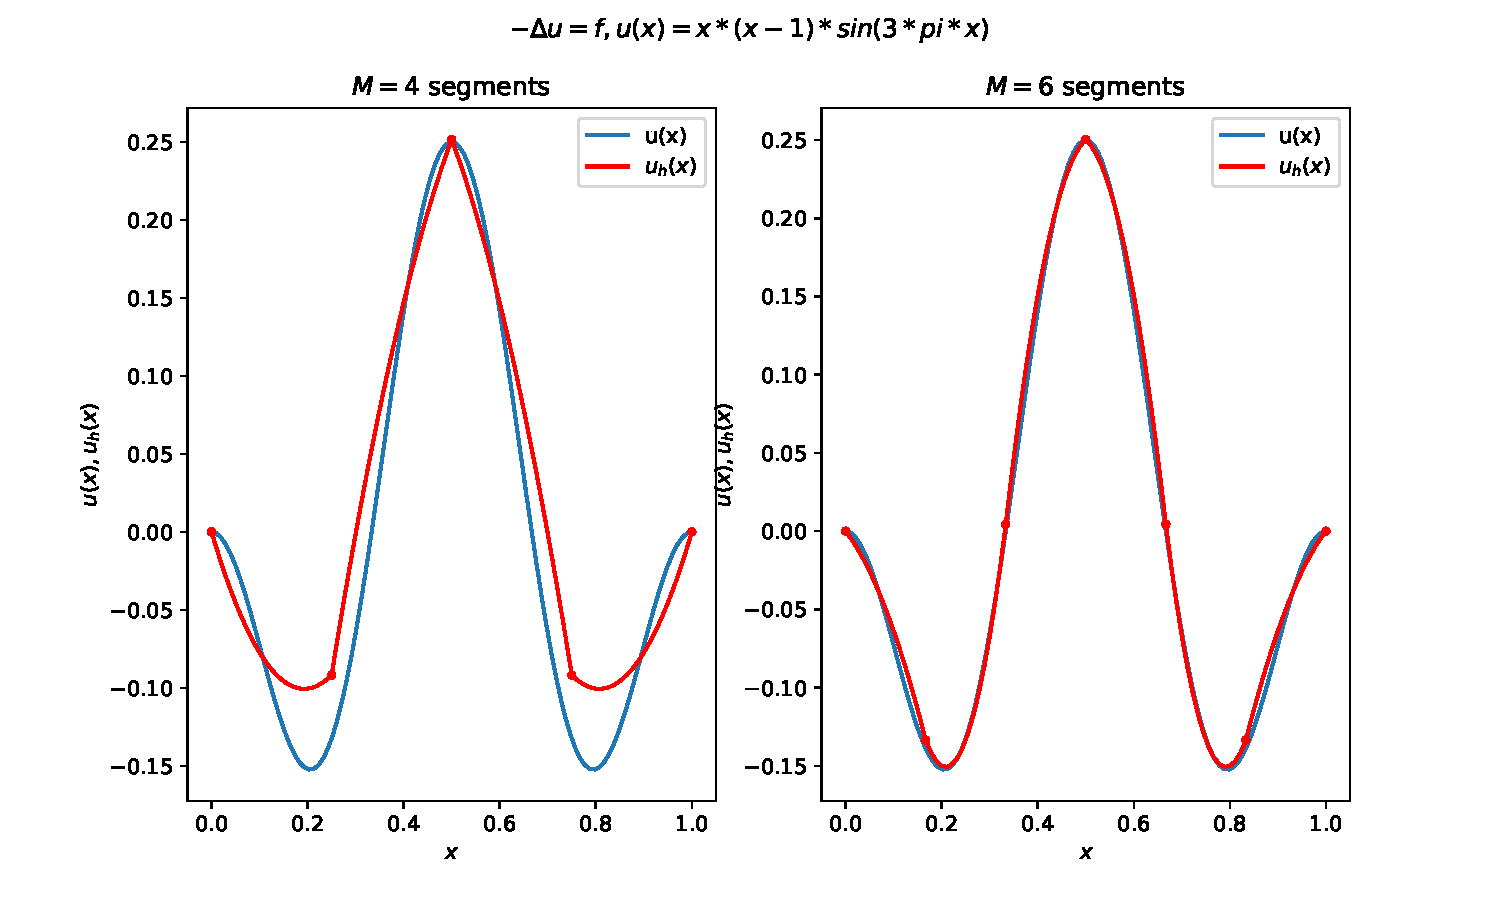
\includegraphics[width=\textwidth]{Images/plots/task1_test_sol1.pdf}
  \caption{The blue graphs shows the exact solution.
  The red graphs are the numerical solution for two
different partitions of the domain.
The approximated solution \( u_h \) is sampled at \( 100 \)
equidistant points.}
  \label{fig:test_eq1}
\end{figure}

\begin{figure}
  \centering
  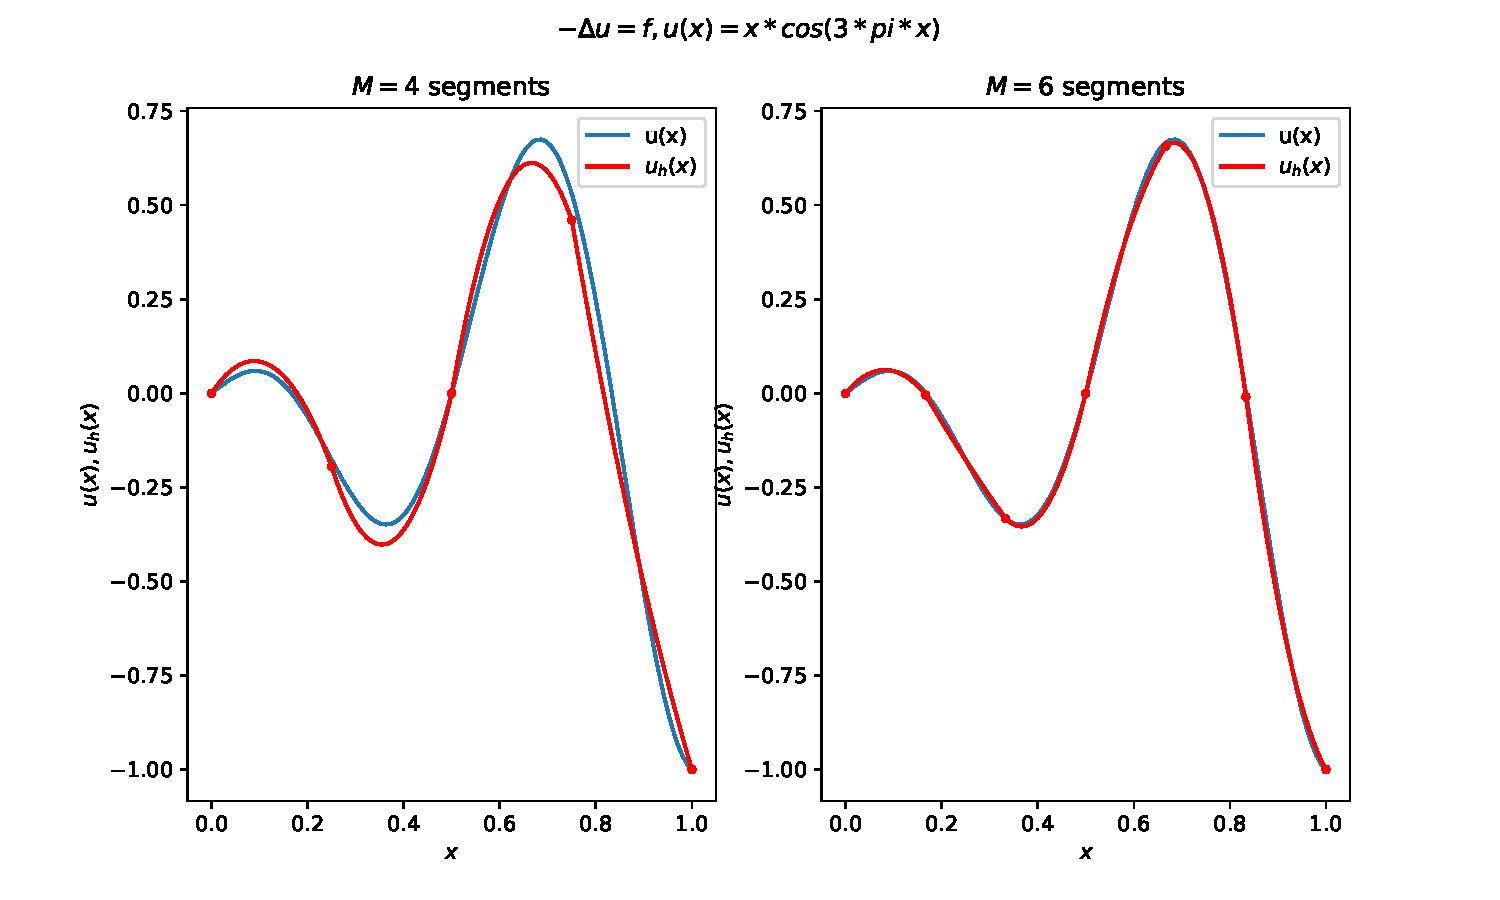
\includegraphics[width=\textwidth]{Images/plots/task1_test_sol2.pdf}
  \caption{The blue graphs shows the exact solution.
  The red graphs are the numerical solution for two
different partitions of the domain.
The approximated solution \( u_h \) is sampled at \( 100 \)
equidistant points.}
  \label{fig:test_eq2}
\end{figure}

\subsection{Convergence analysis}

\begin{theorem}
    Let $u \in H_0^3(\Omega)$ and $u_h \in X_h^2 \cap H_0^1$ be the solutions of the infinite and finite dimensional
    variational problem respectively, where $h$ is the maximum element size in $X_h^2$. Assume further that $F$ in the variational problem is bounded,
    and that $u$ has a second order polynomial interpolant $u_h^2$ on $\Omega$. Then
    \begin{equation}
        ||u - u_h||_{H^1} \leq Ch^2
    \end{equation}
    for some constant $C > 0$.
\end{theorem}
\begin{proof}
  We first note that $a(u, v)$ is both bounded and coercive. Combined with the assumption that $F$ is bounded, we then get from the Lax-Milgram theorem (\cite{CC}, page 15)
    that the variational problem admits a unique solution.
    
    From Cea's lemma (\cite{CC}, page 18) we then obtain
    \begin{equation}
        ||u - u_h||_{H^1} \leq \frac{M}{\alpha}||u - v_h||_{H^1} = \frac{M}{\alpha}(||u - v_h||_{L^2} + |u - v_h|_{H^1}) \quad \forall v_h \in X_h^2 \cap H_0^1.
    \end{equation}
    Since $u(0) = u(1) = 0$, and $\{0, 1\}$ are nodes of the interpolating polynomial, we obtain that $u_h^2(0) = u_h^2(1) = 0$ as well.
    In particular we get that $u_h^2 \in X_h^2 \cap H_0^1$.
    
    Choosing $v_h = u_h^2$ in Cea's lemma results in 
    \begin{equation}
        ||u - u_h||_{H^1} \leq \frac{M}{\alpha}(||u - u_h^2||_{L^2} + |u - u_h^2|_{H^1}),
    \end{equation}
    which combined with lemma 4.4 (\cite{CC}, page 19) gives us
    \begin{equation}
        \begin{aligned}
            \frac{M}{\alpha}||u - v_h||_{H^1} &\leq \frac{M}{\alpha}(C_{2}h^3|u|_{H^3} + C_{1}h^2|u|_{H^3}) \\
            &= h^2\frac{M}{\alpha}(C_{2}h|u|_{H^3} + C_{1}|u|_{H^3}) \\
            &= Ch^2
        \end{aligned}
    \end{equation}
\end{proof}

\subsubsection{Numerical Verification}

To numerically calculate the \( \mathcal{L}^2 \) and \( \mathcal{H}^1 \) norm
we write the integral as a sum over the elements
and use a change of variables similar to the stiffness matrix.
The inner integrals have to be calculated numerically.

\begin{align}
  \lVert u - u_h \rVert_{\mathcal{L}^2(\Omega)}^2 
    &= \int_{\Omega}(u(x) - u_h(x))^2 \,\mathrm{d}x \\
    &= \sum_{k=1}^{M} h_k \int_{0}^{1}
    \left(
    u(\Phi_k(\xi)) 
      - \sum_{\alpha=0}^{2} u_{\theta(k, \alpha)} \Psi_{\theta(k, \alpha)}(\xi)
    \right)^2 \,\mathrm{d}x
\end{align}

\begin{align}
  \lvert u - u_h \rvert_{\mathcal{H}^1(\Omega)}^2 
    &= \int_{\Omega}(u'(x) - u_h'(x))^2 \,\mathrm{d}x \\
    &= \sum_{k=1}^{M} h_k \int_{0}^{1}
    \left(
    u'(\Phi_k(\xi)) 
      - \frac{1}{h_k} \sum_{\alpha=0}^{2} u_{\theta(k, \alpha)} \Psi_{\theta(k, \alpha)}'(\xi)
    \right)^2 \,\mathrm{d}x
\end{align}

We observe in figure \ref{fig:conv_plot} that the convergence orders
match the theoretical results. The equation used is the same as our
first test equation (see figure \ref{fig:test_eq1}).

\begin{figure}
  \centering
  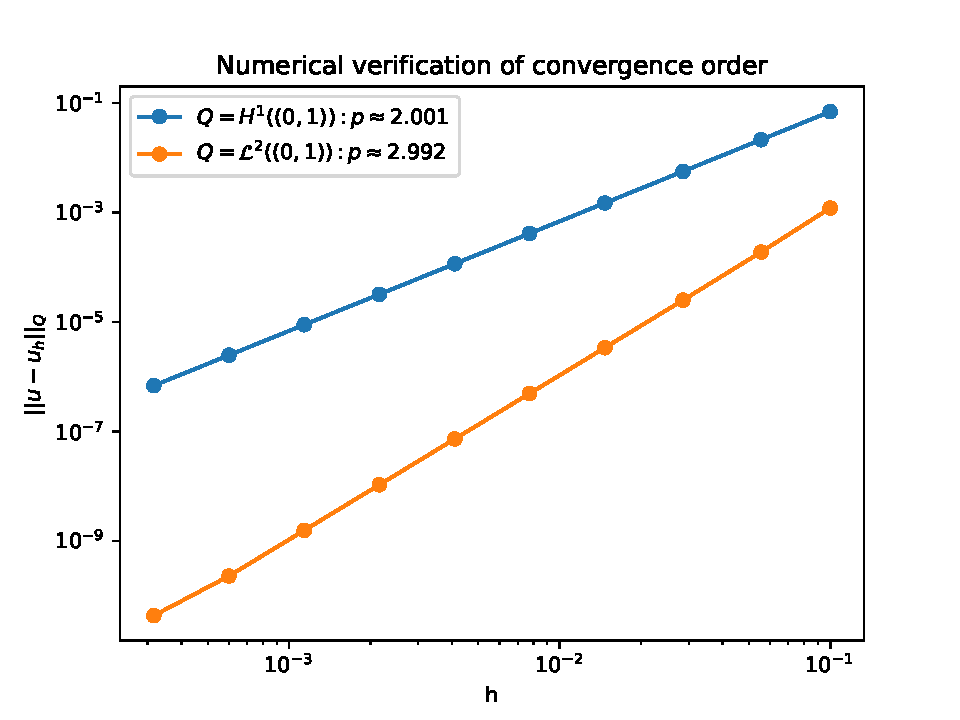
\includegraphics[width=0.75\textwidth]{Images/plots/task1_conv_plot.pdf}
  \caption{Convergence plot for the test solution
  \( u(x) = x(x-1)\sin(3\pi x) \) in both
  \( \mathcal{L}^2 \) and \( \mathcal{H}^1 \) norm.
\( h \) is the element size for a equidistant partition of \( (0, 1) \).}
  \label{fig:conv_plot}
\end{figure}

\subsection{Generalisation}

We have used the second order Lagrange finite elements
throughout this project. The source code is written
such that any degree \( d \) of Lagrange basis functions can be used.
The process here is effectively to replace every 
\( 2 \) in section \ref{sec:sec} with \( d \).

